\section{Data and scoring parameters}\label{app:data}

\begin{table}[h]\centering\small
\caption{Corpus, scoring, and samples in one place. Full construction
detail, the per-class breakouts, and all demoted analyses are in the
supplementary material and the online appendix.}
\label{tab:data}
\begin{tabular}{p{4.2cm}p{9.2cm}}
\toprule
Corpus & USPTO Trademark Annual Applications backfile (TRTYRAP): 13.99
million case files, 1884--2025, re-parsed to 242 million dated
prosecution events. \\
Theme model & LDA, $T = 50$, fitted once on a stratified sample of
448{,}437 filings across all 45 Nice classes; vocabulary of 62{,}168
unigrams and bigrams; resolutions 500 (global) and 50 (per class) refit
for Section~\ref{sec:three_scorings}. \\
References & Per-filing windows of 1{,}826 days on each side of the
filing date, same-class filings only, flat weighting; a filing with fewer
than 500 same-class filings on either side is unscored. Scoring years
1995--2019. \\
Registration sample & 9.02 million scored class-records filed 1995--2018. \\
Five-year-proof sample & 3.10 million unique scored registrations issued
2002--2018; failure is a dated \S8/\S71 cancellation at registration age
4.0--8.5 years. \\
Firm samples & 2.07 million registered debut filings 1995--2018 (SEC
reporting); 999{,}442 debut owners 2009--2018 (funding ladder). \\
Owner links & SEC registrants and Form~D issuers by normalized exact
name; PatentsView assignees likewise. \\
\bottomrule
\end{tabular}
\end{table}

The burn-in cut at 1995 is set empirically: thin past references inflate
past-facing surprise, and the measured contamination falls below any
interpreted effect size from 1993, so the 1995 cut is conservative by
about two years (Figure~\ref{fig:burnin}).

\begin{figure}[h]\centering
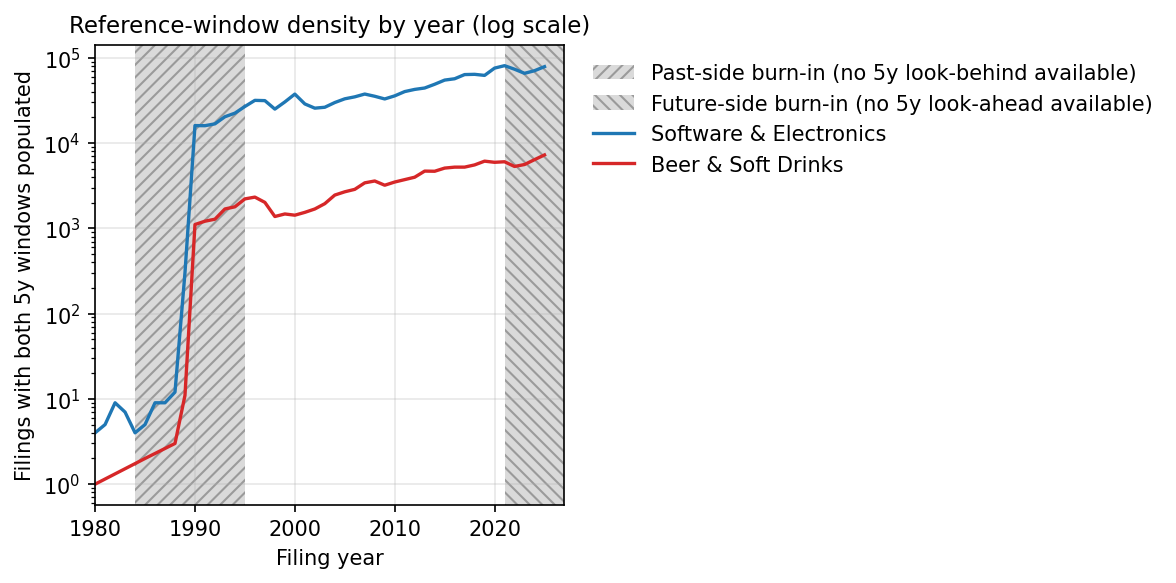
\includegraphics[width=0.85\textwidth]{results/burnin.png}
\caption{Reference-window density by year on log scale. Hatched regions
are the past-side and future-side burn-in zones where the five-year
window is incomplete; the dotted line marks the 1995 analysis cut.}
\label{fig:burnin}
\end{figure}
